\documentclass[a4paper,11pt,twoside,openright]{Thesis}

\usepackage[japanese,master]{ThesisTemplate} 
%% オプション"japanese"を消すと英語化されます。
%% 論文種類は、phd, master, bachelor の3種類です。(デフォルトはphd)

\setcounter{secnumdepth}{3} % show subsubsection numbers

\putTitle{HL-LHC ATLAS実験に向けたシリコンピクセル検出器の粒子線に対する応答評価試験}
\putAuthor{鷲津 優維}{お茶の水女子大学 人間文化創成科学研究科 理学専攻}
\date{\today}

\begin{document}
\maketitle
\frontmatter
\putAbstract{inputs/abst}
\tableofcontents

\mainmatter
\chapter*{序論}
Large Hadron Collider(LHC)は欧州原子核研究機構(CERN)に設置された,重心系エネルギー13TeVの世界最大の陽子陽子衝突型の粒子加速器である.LHCの4つの衝突点のうちの1つに設置されたATLAS検出器を用いて,素粒子標準模型の精密測定および,それを超えた物理の探索を行なっている実験がATLAS実験である.2026年の開始を目指して,LHCの高輝度計画・High-Luminosity LHC(HL-LHC)計画が進められている.LHCのルミノシティを向上させることで,統計量が増えるため,超対称性などの様々な模型が予想する新粒子への感度が向上し,重い粒子の探索が可能になることが期待されている.このHL-LHC計画に伴い,ATLAS検出器の内部飛跡検出器は,受ける放射線量の増加,検出器のヒット占有率の増加などに対応するために,Inner Tracker(ITk)と呼ばれるシリコン検出器への総入れ替えが予定されている.\par
この総入れ替えのために,内部に用いるピクセルセンサモジュールを世界で約6800個制作する必要がある.日本グループはそのうちの約2000個を担当する予定である.ここでは,フレキシブル(Flex)基板,フロントエンド集積回路(ASIC),シリコンピクセルセンサの3要素で構成された検出器をピクセルセンサモジュールと呼ぶ.センサとASICはバンプボンディングと呼ばれる手法,ASICとFlex基板はワイヤボンディングと呼ばれる手法で接続されている.量産されたモジュールは品質性能基準を達成しているか確認するために,様々な試験にかけられる.\par
本研究では,この試験項目の1つである,粒子線に対する応答評価試験を取り扱った.この試験は,ASICとセンサ間のバンプボンディングの部分に異常がないかを確認する試験である.HL-LHCのために開発されたASICのピクセルサイズは$50\times50 \mathrm{\mu m^2}$で,ピクセルセンサの信号が電極を通して個別にASICのピクセルで処理されるため,このバンプボンディングに異常があると,信号を伝えることができず,正常なデータを取得することができない.この試験には2つの手法があり,モジュールに粒子が入射した時の信号のタイミングでデータ取得を行うセルフトリガと呼ばれる手法と,シンチレータを用いて,シンチレータに粒子が入射した時の信号のタイミングでデータ取得を行う外部トリガと呼ばれる手法がある.本研究では,応答評価試験方法の確立のために必要なファームウェア,ソフトウェアを開発した上で,粒子線に対する応答評価試験のデータを2つの手法で取得し,実際に応答評価試験を行うことができるかどうかの確認・考察,2つの手法それぞれの利点欠点を比較した.\par
本論文では,第1章で,現在のLHC ATLAS実験と2024年以降に予定されているHL-LHC計画に伴うATLAS検出器のアップグレードについて,第2章で,アップグレードに伴うモジュールの量産と,モジュールの構成について,第3章で,応答評価試験をするにあたって作成したファームウェアの動作確認の様子,第4章で,セルフトリガによる応答評価試験,第5章で,外部トリガによる応答評価試験,第6章で,2つの手法で取得したデータからわかるそれぞれの利点欠点比較を述べている.

\chapter{アップグレードに向けたモジュール量産}
前章で述べたように,HL-LHC計画に伴い,内部飛跡検出器のアップグレードが計画されている.本章では,それに伴う,モジュールの量産について説明し,モジュールの構成,要素であるシリコンセンサの原理,フロントエンドASICについて述べ,モジュールの量産について必要な試験項目について説明する.

\section{モジュール量産}
HL-LHC計画にあたって,内部飛跡検出器の総入れ替えを予定しているため,内部に用いるピクセルモジュールの量産が必要である.世界で約10000個のモジュールの量産が計画されており,日本グループはそのうちの約2000個を担当する予定になっている.\\
現在は,実機で用いるモジュールを量産するための準備として,プロトタイプ版のモジュールで量産体制の確認が計画されている.プロトタイプ版のモジュールは2月ごろに完成が予定されている.

\section{ピクセルモジュールの構成}
この節では,ピクセル検出器の構成について説明する.以下にピクセル検出器の構造図を示す.ピクセル検出器はFlex基板,フロントエンドASIC,シリコンピクセルセンサの3要素で構成されている.


\section{シリコンピクセルセンサ}
この節では,ピクセル検出器を構成する要素の1つであるシリコンピクセルセンサについて説明する.

\subsection{シリコンピクセルセンサの原理}
シリコンセンサの動作原理は半導体に従う.この節では,半導体の基本原理と性質について述べる.
物質は導体,絶縁体,半導体の3種に分類することができる.これは,電気抵抗値によって決まっており,半導体は導体と絶縁体の中間の値をもつ.一般に室温で,$10^{-2}$から$10^9 \mathrm{\Omega cm}$の範囲に分類される.典型的な半導体物質にはシリコン,ゲルマニウム,ガリウムヒ素などがあげられる.

\subsubsection*{pn接合と空乏化}
高純度の半導体は,電気を通しにくいが,不純物を添加(ドープ)することによって電気的特性を変えることができる.ホウ素などの3価の元素をドープする場合,これをp型半導体と称する.p型半導体では,価電子帯に電子の欠損である正孔が生じ,これが電気伝導に寄与する.一方ヒ素やリンなど5価の元素をドープする場合は,n型半導体と称する.n型半導体では自由電子が発生し,これが電気伝導に寄与する.p型半導体における不純物をアクセプタ,n型半導体における不純物をドナーと呼ぶ.\\
一般的な半導体検出器は,n型とp型の半導体を接合(pn接合)した構造をもつ.以下の図のよう,n型とp型の接合面付近では,電子-正孔が再結合した空乏層が発生する.これに逆電圧$V_b$を印加することによって空乏層を拡張することができる.このときの電圧$V_b$と空乏層の幅$d$の関係は以下のように求められる.接合面を原点,空乏層を$x_p < x < x_n$とし,ある位置での電位を$V$,電荷密度を$\rho_e$とする.また,各半導体のアクセプタ濃度を$N_a$,ドナー濃度を$N_d$とする.素電荷を$e$,シリコンの誘電率を$\epsilon$とする.

\subsubsection*{荷電粒子の検出}
荷電粒子が物質中の電子との衝突によって失うエネルギーは,Bethe Blochの式であらわされる.

\subsubsection*{エネルギーバンド}
孤立した原子では,エネルギー順位は離散的な値をとる.多数の原子が集めると原子同士の引力と斥力の混じった相互作用により,位置に依存する連続的なバンド状順位をみなすことができる.これをエネルギーバンドという.エネルギーバンド構造は,価電子帯,禁制帯,伝導体から構成される.絶縁体・半導体・導体の違いはこのエネルギーバンド構造の違いによるものである.導体では,バンドが重なっているため,電子やホールといった電荷のキャリアが自由に動くことが可能である.一方で,半導体や絶縁体では,バンド間にギャップがあるため,自由に動くことができない.半導体の場合は,このギャップ幅が$\mathrm{eV}$オーダーであり,熱的な励起によってギャップを超えることが可能になる.絶縁体の場合は,ギャップ幅が約4$\mathrm{eV}$より大きく,室温においてキャリアが自由に動くことができない.

\subsubsection*{ドナーとアクセプタ}


\subsection{バイアス構造}
シリコンピクセルセンサには,製造時に良品不良品を選別するための高電圧用のバイアス構造が備わっている.\\
バンプボンディングの前にセンサのみの試験を行い,動作不良センサを取り除く品質評価の工程がある.このピクセルセンサ評価方法として,IV測定がある.IV測定には全てのピクセルがGNDに落とされている必要があり,また,各ピクセルは分離されている必要がある.そのために必要になるのがバイアス構造である.バイアス構造は,ピクセル間にバイアスレールを置き,そこから各ピクセルにバイアス抵抗を引く.この構造により,ピクセルはGNDと同電位とすることができ,また,各ピクセルが抵抗により,分離される.

\subsection{今回使用したシリコンピクセルセンサ構造}
本論文で扱うピクセルセンサの表面構造について述べる.上から見たセンサの様子である.ピクセルセンサは2次元的に電極が配列されており,センサのみのテストのためにバイアスレールが敷かれている.

\section{HL-LHC ATLAS実験用新型ASIC・RD53A}
この節では,ピクセル検出器からの信号は,検出器に直接接続された電気回路で最初に処理される.この電気回路をフロントエンドエレクトロニクスと呼ぶ.この回路は,全て専用の信号読み出し用ASIC内に実装されている.そのため,フロントエンドASICと呼ぶこともあるが,以降ではASICと呼ぶことにする.\\
この回路を用いて検出器からの微弱な電気信号を受け取り,計測用のシステムに最適化した応答をするように信号をアンプ回路や波形整形回路などで調整する.さらに,コンピュータでの解析処理や,データの保存のためにアナログ信号をデジタル信号に変換する.\\
以下にピクセル検出器と読み出しASICの接続図を示す.ピクセル検出器の各チャンネルとASICはバンプボンディングという手法で接合し,ASICでは検出器からの信号に対して処理を行う.\\


RD53AはHL-LHC ATLAS実験用に開発されたプロトタイプ版の新型ASICであり,前章で述べたような,高い放射線耐性と,高い位置分解能を達成する.以下に現行のATLAS検出器で用いられているASIC・FEI4とFEI3,プロトタイプ版新型ASIC・RD53Aの比較を示す.

\begin{table}[h]
  \centering
  \caption{現行のASIC2種と新型プロトタイプ版ASICの比較}
  \begin{tabular} {|l|cc|c|} \hline
    ASIC名 & FEI3 & FEI4 & RD53A \\ \hline \hline
    ピクセルサイズ & 50 $\times$ 400 $\mathrm{\mu m^2}$ & 50 $\times$ 250 $\mathrm{\mu m^2}$ & 50 $\times$ 50 $\mathrm{\mu m^2}$ \\
    ピクセルのチャンネル数 & 18 $\times$ 160 & 80 $\times$ 336 & 50 $\times$ 50 $\mathrm{\mu m^2}$ \\ 
    チップサイズ & 7.6 $\times$ 10.8 $\mathrm{mm^2}$ & 20.2 $\times$ 19.0 $\mathrm{mm^2}$ & 20 $\times$ 11.8 $\mathrm{mm^2}$\\ \hline
  \end{tabular}
  \label{tab:ASIC}
\end{table}

このように,RD53Aは現行のASICと比較してピクセルサイズが小さいため,高い位置分解能を達成する.

\subsection{レジスタ}
ASICには,アナログ回路とデジタル回路の振る舞いを調節するために,回路の動作を制御する設定値を保持するレジスタが存在する.RD53Aのレジスタは2種類存在し,全てのピクセルに共通の設定を保存するグローバルレジスタ(GR)と各ピクセルの設定値を保持するピクセルレジスタ(PR)がある.
\begin{itemize}
\item グローバルレジスタ\\
  RD53Aには137個のGRがあり,ピクセルに共通が閾値(threshold),回路のオンオフなどを設定することができる.
\item ピクセルレジスタ\\
  Synchronus Frontendには3 $\mathrm{bit}$,その他の2つのフロントエンドには8 $\mathrm{bit}$のレジスタがある.ピクセルのデジタル回路のオンオフや閾値(threshold)を設定することができる.
\end{itemize}


\subsection{RD53Aフロントエンドデザイン}
RD53Aはプロトタイプ版のため,Synchronase Frontend, Linear Frontend, Differential Frontendと,3つの異なるフロントエンドデザインが存在する.

\begin{figure}[h]
\centering
\includegraphics[width=8cm]{./figure/RD53A_FE.png}
\caption{RD53Aのフロントエンドデザイン}
\label{fig:RD53AFE}
\end{figure}

今回は実機で利用されることが予定されているDifferential Frontend(以下:Diff FE)のみを用いて研究を行なったため,それについて詳しく説明する.

\subsubsection*{Diff FEの仕組み}
3つのフロントエンドで大きく異なるのは,アナログ回路部分の構造である.Diff FEのアナログ回路構造を以下に示す.\\

\begin{figure}[h]
\centering
\includegraphics[width=8cm]{./figure/RD53A_DiffFE.png}
\caption{Diff FEのアナログ回路構造}
\label{fig:DiffFE}
\end{figure}

図\ref{fig:DiffFE}に示したように,Diff FEでは,RD53AのGR値である''DiffVthin1''と''DiffVthin2''で閾値を設定可能である.これらのGR値は,入力された信号(\ref{fig:DiffFE}の赤い信号)と,それに対して反転増幅を行なった後の信号(\ref{fig:DiffFE}の青い信号)それぞれに作用するオフセット電圧である.Diff FEはこれらの信号の差動によって,出力信号を定義しているため,オフセットを変化させることで,閾値を調整することができる.



\subsection{HitOR信号}
RD53Aには,現行のFEI4に実装されているセルフトリガ機能がない代わりに,HitORというセンサに荷電粒子が入射したタイミングで,出力される信号が存在する.HitOR信号出力する仕組みについて説明する.図\ref{fig:HitOR}はRD53Aの一部である$8 \times 8 \mathrm{pixel}$を示している.

\begin{figure}[h]
\centering
\includegraphics[width=8cm]{./figure/HitOR.png}
\caption{HitOR信号のネットワーク図}
\label{fig:HitOR}
\end{figure}

HitOR信号は,図\ref{HitOR}の各ピクセルに割り当てられている番号1-4ごとにまとめて読み出される.これを番号ごとにネットワークと呼ぶ.このネットワークは任意のネットワークに含まれるピクセルの上下に1つのネットワーク,左右に異なる2つのネットワークが存在するように配置されている.例えば,1番のネットワークのあるピクセルには,3番のネットワークが上下に存在し,左右には2番と4番のネットワークが存在するようになっている.このように配置されたネットワークごとに,HitORは読み出される仕組みになっている.

\section{モジュール量産に向けた品質性能試験}
量産されたモジュールは品質性能基準を達成するために,試験にかけられる.その試験項目の1つとして,本論文に関わる,粒子線に対する応答評価試験が存在する.

\subsection{粒子線に対する応答評価試験の意義}
HL-LHC ATLAS実験に向けたピクセル検出器量産に際して,全ての検出器モジュールに対して,品質管理のための試験を行う.この試験項目の1つとして,粒子線に対する応答評価試験(以下:ソーススキャン)が設けられている.\\
前章でも述べたように,ピクセル検出器の各チャンネルとASICはバンプボンディングという手法で接続されている.このバンプボンディングに異常がないかどうかを確認するための試験が,ソーススキャンである.\\

\subsection{応答評価試験の手法}
応答評価試験には,主に2種類の手法がある.1つは,センサに荷電粒子が入射した時の信号を取得したタイミングでデータ取得を行う,セルフトリガと呼ばれる手法.もう1つは,センサの上にシンチレータ,その上に粒子線源を設置し,シンチレータに粒子線が入射した時の信号を取得したタイミングでデータ取得を行う手法である.今回はこれら2種類の手法を用いてソーススキャンを行い,どのような試験結果の振る舞いがなされるかの検証を行なった.\\
今回用いた読み出しASIC・RD53Aには,セルフトリガ機能が実装されていないため,HitOR信号を外部に出力し,FPGAを用いて処理することでデータ取得を行なった.\\
YARRソフトウェアには,外部トリガスキャンという機能が実装されているため,今回はこの外部トリガにHitOR信号を用いた手法をセルフトリガ,シンチレータに粒子線が入射した時の信号を用いた手法を外部トリガと呼ぶ.

\subsection{本研究の目的}
本研究では,シリコンピクセルセンサが接続されたHL-LHC ATLAS実験用新型ASIC搭載モジュールを用いて,2種類の手法で行なったの粒子線に対する応答評価試験結果について報告する.

\chapter{粒子線に対する応答評価試験のための読み出しシステムの動作確認}
この章では,粒子線に対する応答評価試験のために行なった,外部トリガを処理する機能の追加と,応答評価試験のための準備について述べる.

\section{読み出しセットアップ概要}
以下に読み出しシステムの概要を示す.主にRD53A搭載のSingle Chip Card(SCC)とFPGAボード,PCを用いて読み出しシステムを構成している.今回は読み出しASICとFPGAボードは,HPC-mDP変換ボードを用いてケーブルにて接続を行い,FPGA内部でASICからのデータ信号の処理を行なった.また,高速通信用インターフェースでPCとFPGAボードを接続し,データ転送を行なった.\par

\begin{figure}[h]
  \centering
  \includegraphics[width=15cm]{./figure/Setup.png}
  \caption{セットアップ}
  \label{fig:setup}
\end{figure}

\subsection*{PC}
PCからPCIeによって接続されたFPGAボードに制御コマンドを送る.また,FPGAボードからきたデータを整理する.DAQの基本的なソフトウェアとファームウェアはYARRのDAQシステムを用いた.YARRは読み出しシステムの構築と性能向上を目指すオープンソースプロジェクトである.

\subsection*{FPGAボード}
Xilinx, Inc.のKintex-7 FPGA搭載KC705評価ボードを使用.このFPGAボードは,研究室規模の実験で使うことを想定しているため,FPGA評価ボードは一般的に流通してて入手性がよいため,このFPGAボードを使用している.また,KC705はPCIe通信に対応し,PCとPCIe間では5.12 $\mathrm{Gbps}$の通信速度に対応している.今回はYARRのシステムに外部トリガを受信,処理を行う機能を追加し,RD53Aの出力するHitOR信号を用いて,外部トリガを受信できているかを確認した.

\subsection*{アダプタカード}
ASICはDP-mDPケーブルからmDP-HPCアダプタカードを通してFPGAボードに接続される.

\subsection*{RD53A搭載Single Chip Cardモジュール}
ASICを1チップ搭載した試験用モジュールがSingle Chip Cardモジュールである.今回試験したのはアップグレード用のプロトタイプ版ASICであるRD53A搭載のモジュールである.センサ付きのRD53Aが搭載されたモジュールの写真を以下に示す.
RD53Aは細い金属ワイヤにより基板上の回路パターンと電気的に接続されている.基板にRD53Aが外部と通信するためのDPコネクタ(図中:DP1),電源供給のためのmolexコネクタ(図中:PWR IN),センサに電圧を印加するためのLEMOコネクタ(図中:HV),センサが検出した信号を外部に出力するためのDPコネクタ(DP2)が実装されている.
\begin{figure}[h]
  \centering
  \includegraphics[width=7cm]{./figure/rd53a.png}
  \caption{センサ付きRD53A搭載Single Chip Cardモジュール}
  \label{fig:scurve}
\end{figure}

今回電源とセンサに印加した電圧は\ref{tab:voltage}に示す.

\begin{table}[h]
  \centering
  \caption{今回RD53Aとセンサに供給した電圧}
  \begin{tabular} {|l|cc|c|} \hline
     & RD53A & RD53A & ピクセル \\ 
     & アナログ回路 & デジタル回路 & センサ \\ \hline
    印加電圧[$\mathrm{V}$] & 1.80 & 1.80 & -50 \\ \hline
  \end{tabular}
  \label{tab:voltage}
\end{table}


\subsection*{$\beta$線源}
今回は粒子線として$\beta$線源であるストロンチウム90を使用した.ストロンチウム90は中性子過剰であるため,$\beta$崩壊によってイットリウム90を生成し,その後さらなる$\beta$崩壊によってジルコニウム90となる.半減期は28.79年であるが,2段階の$\beta$崩壊が起こるため,$\beta$線のエネルギーは高いものになっている.式\ref{eq:beta}にベータ崩壊の機構を,式\ref{eq:sr90}にストロンチウムの崩壊過程を示す.\par
\begin{equation}
  \label{eq:beta}
  n \rightarrow p^{+} + e^{-} + \overline{\nu_e}
\end{equation}
\begin{equation}
  \label{eq:sr90}
  \ce{^{90}Sr} \rightarrow \ce{^{90}Y} \rightarrow \ce{^{90}Zr}
\end{equation}


$\beta$線の今回用いた$\beta$線源は2017/02/13時点で$ 5.00 \times 10^3 \mathrm{Bq}$のものであった.すなわち現在の放射能は以下のように求められる.

\begin{equation}
\label{eq:radiation}
  A = -\lambda N_1 = A_0 \exp \left( - \frac{\ln 2}{T} t \right)
\end{equation}

ここで,
\begin{description}
\item[] $A_0$:2017/02/13時点での放射能($ 5.00 \times 10^3 \mathrm{Bq}$)
\item[] $T$:\ce{^{90}Sr}の半減期(28.79 $\mathrm{year}$)
\item[] $t$:2017/02/13から現在までの時間(25/12 $\mathrm{year}$)
\end{description}

式\ref{eq:radiation}より,現在の放射能$A$は,$4.76 \times 10^3 \mathrm{Bq}$と求まる.
  

%\begin{table}[h]
%  \centering
%  \caption{今回使用した$\beta$線源の放射能}
%  \begin{tabular}{|l|c|} \hline
%    基準日 & 2017/02/13 \\
%    放射能 & 5.00 $\times 10^3 \mathrm{Bq}$ \\ \hline
%  \end{tabular}
%  \label{tab:beta}
%\end{table}



\section{伝達確認}
ソーススキャンを行うために,既存のKC705用YARRファームウェアに外部トリガを処理する機能を追加した.本節では,機能を追加したファームが外部トリガを受信確認について述べる.

\subsection{コマンド信号とデータ信号の確認}
オシロスコープでコマンド信号とデータ信号をRD53A SCC上でプローブし,波形を確認した.

\subsection{デジタルスキャン}
全ピクセルのデジタル回路に複数回擬似パルスを注入して,注入した回数のうち何回応答が返ってくるのかを確認する.この作業をデジタルスキャンと呼ぶ.全ピクセルごとの回路の応答を確認し,データの転送線,FPGA内部の処理,PCへの通信の各経路でデータの損失がないことを確認するのに有効である.図\ref{fig:digital}に100回擬似パルスを注入した時の応答数の分布を示す.
\begin{figure}[h]
  \centering
  \includegraphics[width=7cm]{./figure/DigitalScan.png}
  \caption{デジタルスキャン}
  \label{fig:digital}
\end{figure}


\subsection{アナログスキャン}
アナログ回路に複数回擬似パルスを注入して,注入した回路のうち何回応答が返ってくるのかを確認した.この作業をアナログスキャンと呼ぶ.今回はDiff FEのみを使用するので,その他のフロントエンドは,グローバルレジスタの''EnCoreColSync1/2'',''EnCoreColEnLin1/2''を全て0にすることで非使用に設定した.また,Diff FE内接続されているピクセルセンサの上下構造の違いにより,上半分にノイズが多く現れるため,それを防ぐために,Diff FEのアナログ回路のLCC回路の部分をオンにする.これは,グローバルレジスタ''DiffLccEn''という値を0から1に変更し,''DiffLcc''を255にすることでオンにすることができる.図\ref{fig:analog1}にLCC回路をオフにした場合,図\ref{fig:analog2}オンにした場合それぞれのDiff FEのアナログスキャンの結果を示す.LCC回路をオフにすると,上部の横端にノイズが多く発生してしまうため,ASICのピクセルが非使用に設定されてしまう.LCC回路をオンにすることで,ノイズの量が減り,センサの面積を有効に利用することができる.

\begin{figure}[h]
  \centering
  \begin{minipage}[b]{0.4\linewidth}
    \centering
    \includegraphics[width=6cm]{./figure/AnalogScan1.png}
    \subcaption{LCC回路をオフ}
    \label{fig:analog1}
  \end{minipage}
  \begin{minipage}[b]{0.4\linewidth}
    \includegraphics[width=6cm]{./figure/AnalogScan3.png}
    \subcaption{LCC回路をオン}
    \label{fig:analog2}
  \end{minipage}
  \caption{アナログスキャン}
\end{figure}


\subsection{閾値のチューニング}
\begin{figure}[h]
  \centering
  \begin{minipage}[b]{0.4\linewidth}
    \centering
    \includegraphics[width=7cm]{./figure/scurve.png}
    \subcaption{注入電荷$V_{cal}$と応答率の関係}
    \label{fig:scurve}
  \end{minipage}
  \begin{minipage}[b]{0.4\linewidth}
    \includegraphics[width=7cm]{./figure/ThreDiff.png}
    \subcaption{チューニング前後閾値分布}
    \label{fig:ThrDistBefore}
  \end{minipage}
  \caption{閾値チューニング}
\end{figure}

閾値とはピクセルの応答率が50$\mathrm{\%}$となる電荷量で定義され,閾値が目標値になるように各ピクセルのDAC値を調節する作業を閾値のチューニングという.信号が閾値を超えたかあどうかでヒットと認識するかどうかの判定を行なっているが,信号には正規分布に従うノイズが載るため,信号がヒットとして認識される閾値には幅がある.そのため,注入電荷を変化させながら,各ピクセルに試験電荷を複数回入射したときの応答数の関係は,図\ref{fig:scurve}のような曲線になる.この曲線をSカーブと呼び,これを誤差関数でフィッティングすることで,応答率が50 $\mathrm{\%}$となる閾値を求める.
\begin{eqnarray}
  f(Q_{inj}) &=& \frac{1}{2} \left( 1 + \rm{erf} \left( \frac{Q_{inj} - Q_{thr}}{\sqrt{2} \sigma} \right) \right) \\
  \rm{erf}(x) &=& 1- \frac{2}{\sqrt{\pi}} \int^x _0 e^{-t^2} dt
  \label{eq:scurve}
\end{eqnarray}


閾値チューニング前後の各ピクセルの閾値のヒストグラムを図\ref{fig:ThrDistBefore}に示す.目標値は2500$\mathrm{e}$と設定した.2500$\mathrm{e}$という閾値は,センサの厚みとノイズ信号の大きさを考慮した値である.今回使用したセンサの厚みは,150 $\mathrm{\mu m}$であり,式\ref{eq:thr}の厚み300 $\mathrm{\mu m}$の場合のおよそ$1/2$であるため,全て空乏化した場合に発生する信号は10000 $\mathrm{e}$である.まず,この信号をASICが読み出す際に,4分割されてしまったとしても,検出してほしいために閾値は2400 $\mathrm{e}$以下であることが望ましい.また,ノイズ$\sigma$の大きさに対して6-7 $\sigma$離れている必要があるため,バイアスレール有りの場合,$\sigma = 200 \mathrm{e}$と知られているため,1200 $\mathrm{e}$以上にすることが望ましい.閾値のヒストグラムを見ると,1200 $\mathrm{e}$にチューニングした場合は,1200 $\mathrm{e}$以下まで多く分布してしまっているため,今回は分布が1200 $\mathrm{e}$以上に収まるような,2500 $\mathrm{e}$を目標値としてチューニングを行なった.

\subsection{ノイズスキャン}
任意の周波数でトリガを発行し,その全トリガ数に対するのアナログ回路から何回応答が返ってくるのかを確認する.この作業をノイズスキャンと呼ぶ.ピクセルセンサが粒子線以外の信号に対して反応していないことを確認するために有効である.\par
この作業によって,粒子線以外の信号に対して反応している部分は非使用に設定される.引き続きDiff FEのみを使用した.任意の周波数でトリガを送り,その時のアナログ回路からの応答に対して,閾値を超えるものを非使用に設定する.この作業をノイズスキャンと呼ぶ.今回は20000 $\mathrm{Hz}$で5分間ノイズスキャンを3回行なった.以下にノイズスキャンを行う前と行なった後のOccupancy MapとEnable Pixel Mapを示す.

\begin{figure}[h]
  \centering
  \begin{minipage}[b]{0.3\linewidth}
    \centering
    \includegraphics[width=5cm]{./figure/DigitalScan.png}
    \subcaption{ノイズスキャン前のOccupancy Map}
    \label{fig:scurve}
  \end{minipage}
  \begin{minipage}[b]{0.3\linewidth}
    \centering
    \includegraphics[width=5cm]{./figure/DigitalScan.png}
    \subcaption{ノイズスキャン後のOccupancy Map}
    \label{fig:ThrDistBefore}
  \end{minipage}
  \begin{minipage}[b]{0.3\linewidth}
    \centering
    \includegraphics[width=5cm]{./figure/DigitalScan.png}
    \subcaption{以降使用したピクセルの分布}
    \label{fig:scurve}
  \end{minipage}
  \caption{閾値チューニング}
\end{figure}


\subsection{HitOR信号の伝達確認}
モジュールの上に$\beta$線源を配置し,オシロスコープでHitOR信号をRD53A SCC上でプローブすることで,波形を確認した.また,FPGAまでHitOR信号が伝わっているかどうか,正常に処理され,そのタイミングでトリガが出力されているかどうかをVivadoのLogic Analyzerを用いて確認した.それが以下の図である.



このようにファームウェアに外部トリガを取得し,処理する機能を追加できていることを確認した.







\chapter{セルフトリガを用いた応答評価試験}
この章では,セルフトリガを用いた粒子線に対する応答評価試験について述べる.\ref{sec:selfsetup}節で応答評価試験セットアップ,\ref{sec:latency}節で粒子線を用いた応答評価試験のために必要だったLatency Scan機能について述べ,そのあとに,\ref{sec:selfhow}節で手順,\ref{sec:selfconc}節で取得データの結果を示し,\ref{sec:selfsum}節で考察を行なっている.

\section{セルフトリガを用いた応答試験セットアップ}
\label{sec:selfsetup}
この節では,セルフトリガによる応答評価試験のセットアップについて述べる.主なセットアップは読み出しシステムの動作確認時の図\ref{fig:setup}と変わらず,RD53A搭載のSingle Chip Card(SCC)とFPGAボード,PCを用いて読み出しシステムを構成し,SCCとFPGAボードはアダプタカードを用いてディスプレイポートケーブルによって接続した.その様子を図\ref{fig:selfsetup}に示す.センサからの信号を外部に出力するためのコネクタをアダプタカードのport D,FPGAがRD53Aからのデータを受け取るためのコネクタをアダプタカードのport Aに繋ぐようにしている.また,モジュールの上に$\beta$線源を配置した.

\begin{figure}[h]
  \centering
  \includegraphics[width=12cm]{./figure/selfsetupcab.png}
  \caption{セルフトリガを用いた応答評価試験セットアップ配線図}
  \label{fig:selfsetup}
\end{figure}

\subsection*{$\beta$線源}
今回は粒子線として$\beta$線源である\ce{^{90}Sr}を使用した.\ce{^{90}Sr}は中性子過剰であるため,$\beta$崩壊によって\ce{^{90}Y}を生成し,その後さらなる$\beta$崩壊によって\ce{^{90}Zr}となる.半減期は28.79年であるが,2段階の$\beta$崩壊が起こるため,$\beta$線のエネルギーは約$0.545908 \mathrm{MeV}$と高いものになっている.式\ref{eq:beta}にベータ崩壊の機構を,式\ref{eq:sr90}に\ce{Sr}の崩壊過程を示す.2段階で崩壊する時の娘核の放射能は同じになることを考慮し,放射能の計算を行なった.\par
\begin{equation}
  \label{eq:beta}
  n \rightarrow p^{+} + e^{-} + \overline{\nu_e}
\end{equation}
\begin{equation}
  \label{eq:sr90}
  \ce{^{90}Sr} \rightarrow \ce{^{90}Y} \rightarrow \ce{^{90}Zr}
\end{equation}


$\beta$線の今回用いた$\beta$線源は2017/02/13時点で$ 5.00 \times 10^3 \mathrm{Bq}$のものであった.すなわち現在の放射能$A$は式\ref{eq:radiation}で求められる.

\begin{equation}
\label{eq:radiation}
  A = -\lambda N_1 = A_0 \exp \left( - \frac{\ln 2}{T} t \right)
\end{equation}

ここで,
\begin{table}[h]
  \centering
  \begin{tabular}{cc} \hline
    $A_0$ & 2017/02/13時点での放射能($ 5.00 \times 10^3 \mathrm{Bq}$)\\
    $T$ & \ce{^{90}Sr}の半減期(28.79 $\mathrm{year}$)\\
    $t$ & 2017/02/13から現在までの時間(25/12 $\mathrm{year}$)\\ \hline
  \end{tabular}
\end{table}


式\ref{eq:radiation}より,現在の放射能$A$は,$4.76 \times 10^3 \mathrm{Bq}$と求まる.
  


\section{Latency Scan機能の追加}
\label{sec:latency}
この節では,粒子線に対する応答評価のために必要だったLatencyチューニング機能について述べる.

\subsection{YARRにおけるトリガDAQとLatencyの意義}
Latency Scan機能を説明する前に,YARRにおけるトリガDAQについて説明する.YARRソフトウェアを用いたデータ取得におけるトリガDAQについての図を図\ref{fig:YARRDAQ}に示す\par
\begin{figure}[h]
  \centering
  \includegraphics[width=16cm]{./figure/DAQ_sigfig.png}
  \caption{YARRトリガDAQ:配線図(左)とそれに対応する信号(右)を示す.}
  \label{fig:YARRDAQ}
\end{figure}

図\ref{fig:YARRDAQ}の左が配線図を示し,その番号に対応した信号が伝達される様子を右図に示している.\par
\begin{itemize}  
\item まず荷電粒子がセンサに入射した時の信号は図\ref{fig:YARRDAQ}の$\textcircled{\scriptsize1}$SignalのようにASICに入力される
\item 入力されたアナログ信号は,閾値と比較されることで,$ \textcircled{\scriptsize2} $Hitのようなデジタル信号に変換される.
\item 変換されたデジタル信号は,図\ref{fig:YARRDAQ}の左下の配線を介して,データとして保存される部分と,HitOR Outから信号が出力される部分両方に入力される.データとして保存される部分では,Hitを検出したピクセル位置やToT値,Latency値が記録される.一方で,Hit信号がHitOR Outから出力される部分に入力すると,図\ref{fig:YARRDAQ}の左上のHitOR Outから信号が出力され,ケーブルを介して$ \textcircled{\scriptsize3} $のようにFPGAボードに入力する
\item FPGAで信号がトリガとして処理され,$ \textcircled{\scriptsize4} $Triggerとして出力される.
\end{itemize}

RD53Aにトリガが入力された時にどれだけの時間遡ってメモリから情報を読み出すかを定める値がLatencyである.このLatencyがずれていると,データを正しく読み出すことができない.YARRでは,指定されたLatency分遡ったClockの前7 $\mathrm{Clock}$,後8 $\mathrm{Clock}$,計16 $\mathrm{Clock}$分のデータを読み出す.16 $\mathrm{Clock}$の中で何 $\mathrm{Clock}$目のデータであるかを示す値として,L1IDというものが記録される.アナログスキャンにおけるL1IDの分布を以下に示す.\par
\begin{figure}[h]
  \centering
  \includegraphics[width=8cm]{./figure/l1dist.png}
  \caption{アナログスキャンの時のL1IDの分布}
  \label{fig:YARRDAQ}
\end{figure}

理想的にはL1IDが7のところにトリガの中心を合わせたい.そのために,YARRで指定できるLatencyに関する2種類のパラメータを以下に示す.

%\subsubsection*{ソフトウェアで設定されている''delay''}
%擬似パルスを送られてからどれくらい遅れてトリガを出力するかを決める値.前章で述べたデジタルスキャンやアナログスキャンの際に関係し,擬似パルスではなく外部からのトリガを使用してデータ取得するセルフトリガや外部トリガを用いたデータ取得の時には無関係.
%

\subsubsection*{a. ファームウェアの設定値''delay''}
図\ref{fig:YARRDAQ}のaで示されている部分.FPGAからトリガをどれだけ遅れて出力するかを決める値.本論文では,外部からトリガを受け取ってからどれくらい遅延させてFPGAからRD53Aにトリガを出力するかを決める値.

\subsubsection*{b. グローバルレジスタ''LatencyConfig''}
RD53Aの全てのピクセルに共通する設定値であるグローバルレジスタの内の1つにLatencyConfigというLatencyに関する設定値が存在する.LatencyConfigがどのような値であるか説明する図を以下に示す.\par
ASICのあるピクセルが信号を検知すると,そのピクセルが40 $\mathrm{MHz}$のClockに合わせてカウントを始める.そして,FPGAから送られてくるトリガを受け取った時に,そのカウントが設定した''LatencyConfig''の値と等しいピクセルの情報を読み出すようになっている.''LatencyConfig''は,9bitの値であり,0-511まで変化させることが可能である.

\subsection{Latency Scan機能}
前節で述べたように,Latencyが合っていないと,データを正しく読み出すことができないので,Latencyを正しい値にすることが,データを正しく読み出す上で大変重要となる.そこで,今回はグローバルレジスタ''LatencyConfig''値を変化させてデータ取得を行うことで,正しいLatency値を導けるような機能をYARRに追加した.それがLatency Scan機能である.\par
今回,HitOR信号でトリガをかけた場合のLatencyを合わせたかったため,図\ref{sec:selfsetup}のセットアップで以下を行なった.
\begin{enumerate}
\item セルフトリガによって100イベントを取得する
\item 取得したデータのL1IDの分布を得る
\item $\mathrm{L1ID} == 7$であるイベント数を記録
\end{enumerate}
以上を0-511の各''LatencyConfig''値に対して行い,''LatencyConfig''値と$\mathrm{L1ID} == 7$だったイベント数の関係を図\ref{fig:latencydist}のように得る.この時にもっともイベント数が多かった''LatencyConfig''値の時にLatencyが合っていると定義した,

\begin{figure}[h]
  \centering
  \includegraphics[width=13cm]{./figure/latencydist.png}
  \caption{''LatencyConfig''値とL1ID $== 7$だったイベント数の関係}
  \label{fig:latencydist}
\end{figure}


\subsubsection*{LatencyScanのピークが幅を持つ理由}
理想的には,Latency Scanを行なった時の分布は,正しいLatency値にのみピークが立つはずであるが,今回の結果はそうはなっていない.理由は2つある.

\begin{itemize}
\item YARRのファームウェアの仕組みとして,RD53Aに向けて出力されるコマンドは160 $\mathrm{MHz}$のClockで32 $\mathrm{bit}$単位で送る必要がある.しかし,RD53AはLHCのバンチ衝突のレートである40 $\mathrm{MHz}$でヒットが生成されることを前提に設計されている.したがって,8BC分のトリガをまとめてファームウェアから出力する必要があるのだが,YARRのファームウェアの仕組みとして,そのタイミングを正確に合わせていないため,前後8 BC分の幅が生じてしまう.
  
%\item YARRの仕組みとして,32bitに1回トリガを発行するかどうかを決めているので,前後8 $\mathrm{Clock}$分の幅が生じる
\item 図\ref{fig:analogop}はDiff FEのアナログ回路の先を示しており,図\ref{fig:DiffFE}の一番右のCompの部分が図\ref{fig:analogop}の一番左のCompに対応する.アナログ回路から出力された信号はフリップフロップ回路に入力される.しかし,その間に寄生容量(図\ref{fig:analogop}の$C_p$)が生じているため,出力のタイミングに前後2 BCの幅が生じてしまう.これがLatency Scanの結果にも影響する.


    %\item アナログアウトプットのキャパシタンスにズレがあるために前後2 $\mathrm{Clock}$分の幅が生じる.これは,アナログスキャンを行なった時のL1IDの分布を見ると,$\mathrm{L1ID} == 7$のところにのみピークが立つのではなく,前後に2 $\mathrm{Clock}$分の幅を持っていることから確認できる.
\end{itemize}

\begin{figure}[h]
  \centering
  \includegraphics[width=8cm]{./figure/analogop.png}
  \caption{Diff FEのアナログ回路の出力}
  \label{fig:analogop}
\end{figure}



\section{セルフトリガによる応答評価試験手順}
\label{sec:selfhow}
\ref{sec:latency}節で述べたLatencyチューニングを行なった結果,''LatencyConfig''の分布が図\ref{fig:latencydist}のように得られたため,今回は''LatencyConfig''の値を211に設定することで,Latencyを合わせた.Latencyを合わせた上で,以下の3つのトリガ生成方法でデータ取得を行う.

\begin{enumerate}
\item 200 $\mathrm{kHz}$でトリガを生成し,データ取得を行う
\item 線源を置かない状態でセルフトリガによるデータ取得を行う
\item 線源を置いた状態でセルフトリガによるデータ取得を行う
\end{enumerate}

%応答評価試験として,センサの上に線源を置いて30分間のセルフトリガによるデータ取得を行なった.また,背景事象の測定として,30分間線源を置かずにセルフトリガによるデータ取得を行なった.

\section{セルフトリガによるデータ取得結果}
\label{sec:selfconc}
3つのトリガ生成方法で得られたデータのトリガ数とヒット数を表\ref{tab:self}に示す.得られたデータを解析した.

\begin{table}[h]
  \centering
  \caption{トリガ生成方法に対する得られたヒット数とトリガ数}
  \begin{tabular} {l|ccc} \hline
    トリガ生成方法 & ランダムトリガ & セルフトリガ(線源なし) & セルフトリガ(線源あり) \\ \hline \hline
    ヒット数 & 1432633 & 3440511 & 3503191\\
    トリガ数 & $6 \times 10^7$ & 4193685 & 4056311 \\ \hline
  \end{tabular}
  \label{tab:self}
\end{table}

\section{考察}
\label{sec:selfsum}

\subsection*{トリガ生成方法と取得されるデータの内容}
3つのトリガ生成方法による取得されるデータの内容の違いについて表\ref{tab:selfdata}に示す.

\begin{table}[h]
  \centering
  \caption{トリガ生成方法と取得されるデータの内容}
  \begin{tabular} {l|ccc} \hline
    & ランダムトリガ & セルフトリガ(線源なし) & セルフトリガ(線源あり) \\ \hline \hline
    トリガ生成方法 & 200 $\mathrm{kHz}$のトリガ & センサの信号でトリガ生成 & センサからの信号でトリガ生成 \\ \hline 
    取得される & 無関係なトリガで & 無関係なトリガで & 無関係なトリガで\\
    データの内容 & 得られるヒット & 得られるヒット & 得られるヒット \\
    & & センサのノイズ & センサのノイズ \\
    & & & 荷電粒子の信号\\ \hline
  \end{tabular}
  \label{tab:selfdata}
\end{table}

よって,線源ありのセルフトリガによって取得されたデータから,無関係なトリガで得られるヒットと,センサのノイズによる影響を除くことで,荷電粒子からの信号を見積りたい.

\subsection*{荷電粒子からの信号の見積もり}
荷電粒子からの信号を見積もるために,各ピクセルが得たヒット数に着目する.i番目のピクセルに対して,表\ref{tab:selfpara}のように値を定める.
  \begin{table}[h]
    \centering
    \caption{i番目のピクセルに対して得られる値}
    \begin{tabular} {l|ccc} \hline
      & ランダムトリガ & セルフトリガ(線源なし) & セルフトリガ(線源あり) \\ \hline \hline
      ヒット数 & $N_{\mathrm{i.bg}}^{\mathrm{random}}$& $N_{\mathrm{i.bg}}^{\mathrm{self}}$ & $N_{\mathrm{i}}^{\mathrm{self}}$ \\
      トリガ数 & $M_{\mathrm{i.bg}}^{\mathrm{random}}$ & $M_{\mathrm{i.bg}}^{\mathrm{self}}$& $M_{\mathrm{i}}^{\mathrm{self}}$\\ \hline
    \end{tabular}
    \label{tab:selfpara}
  \end{table}


この時,$N_{\mathrm{i}}^{\mathrm{self}}$に対して,ランダムトリガによる影響を除いたもの$N_{\mathrm{i.sig'}}^{\mathrm{self}}$と,それに加えてセンサノイズによる影響を除いた$N_{\mathrm{i.sig}}^{\mathrm{self}}$を,それぞれ式\ref{eq:selfphits1},\ref{eq:selfphits}のように表す.$N_{\mathrm{i.sig}}^{\mathrm{self}}$が荷電粒子による信号の見積もりである.
  
\begin{eqnarray}
  \label{eq:selfphits1}
  N_{\mathrm{i.sig'}}^{\mathrm{self}} &=& N_{\mathrm{i}} - \mathrm{i.Random} \\
  \mathrm{i.Random} &=& \frac{N_{\mathrm{i.bg}}^{\mathrm{random}}}{M_{\mathrm{i.bg}}^{\mathrm{random}}} \times M_{\mathrm{i}}^{\mathrm{self}}\\ \nonumber
  \label{eq:selfphits}
  N_{\mathrm{i.sig}}^{\mathrm{self}} &=& N_{\mathrm{i}} - \mathrm{i.Background} \\
  \mathrm{i.Background} &=& \left(\frac{N_{\mathrm{i.bg}}^{\mathrm{self}}}{M_{\mathrm{i.bg}}^{\mathrm{self}}} + \frac{N_{\mathrm{i.bg}}^{\mathrm{random}}}{M_{\mathrm{i.bg}}^{\mathrm{random}}} \right) \times M_{\mathrm{i}}^{\mathrm{self}} \nonumber
\end{eqnarray}

$N_{\mathrm{i}}^{\mathrm{self}}$と$N_{\mathrm{i.sig'}}^{\mathrm{self}}$のヒット数分布の違いを図\ref{fig:selfhitperpix1}に示す.
\begin{figure}[h]
  \centering
  \includegraphics[width=10cm]{./figure/selfhitperpix1.png}
  \caption{$N_{\mathrm{i}}^{\mathrm{self}}$と$N_{\mathrm{i.sig'}}^{\mathrm{self}}$のヒット数分布}
  \label{fig:selfhitperpix1}
\end{figure}

$N_{\mathrm{i}}^{\mathrm{self}}$と$N_{\mathrm{i.sig'}}^{\mathrm{self}}$1ピクセルあたりのヒット数分布の推移を図\ref{fig:selfhitperpix1bfaf}に示す.横軸が$N_{\mathrm{i}}^{\mathrm{self}}$の値で縦軸が$N_{\mathrm{i.sig}}^{\mathrm{self}}$の値を示し,z軸はpixel数を示している.図\ref{fig:selfhitperpix1}より,$N_{\mathrm{i}}^{\mathrm{self}}$と$N_{\mathrm{i.sig'}}^{\mathrm{self}}$の分布にほとんど違いが見られないことや,\ref{fig:selfhitperpix1bfaf}の分布がほぼ線形であることから,補正前後で分布に変化がなく,$N_{\mathrm{i}}^{\mathrm{self}}$の分布にランダムトリガによる影響はほとんどないことがわかる.

\begin{figure}[h]
  \centering
  \includegraphics[width=10cm]{./figure/selfhitperpixbfaf1.png}
  \caption{$N_{\mathrm{i}}^{\mathrm{self}}$と$N_{\mathrm{i.sig'}}^{\mathrm{self}}$のヒット数分布の推移}
  \label{fig:selfhitperpix1bfaf}
\end{figure}

次に,$N_{\mathrm{i}}^{\mathrm{self}}$と$N_{\mathrm{i.sig}}^{\mathrm{self}}$のヒット数分布の違いを図\ref{fig:selfhitperpix}に示す.
\begin{figure}[h]
  \centering
  \includegraphics[width=10cm]{./figure/selfhitperpix.png}
  \caption{$N_{\mathrm{i}}^{\mathrm{self}}$と$N_{\mathrm{i.sig}}^{\mathrm{self}}$ヒット数分布}
  \label{fig:selfhitperpix}
\end{figure}

$N_{\mathrm{i}}^{\mathrm{self}}$と$N_{\mathrm{i.sig}}^{\mathrm{self}}$1ピクセルあたりのヒット数分布の推移を図\ref{fig:selfhitperpixbfaf}に示す.横軸が$N_{\mathrm{i}}^{\mathrm{self}}$で縦軸が$N_{\mathrm{i.sig}}^{\mathrm{self}}$を示していて,$N_{\mathrm{i}}^{\mathrm{self}}$が10 $\mathrm{Hits}$以下の部分は線形であるのに対し,$N_{\mathrm{i}}^{\mathrm{self}}$の値が大きい分布は$N_{\mathrm{i.sig}}^{\mathrm{self}}$では0に分布しているものが多く,センサノイズの影響が大きいことがわかる.
\begin{figure}[h]
  \centering
  \includegraphics[width=10cm]{./figure/selfhitperpixbfaf.png}
  \caption{$N_{\mathrm{i}}^{\mathrm{self}}$と$N_{\mathrm{i.sig}}^{\mathrm{self}}$のヒット数分布の推移}
  \label{fig:selfhitperpixbfaf}
\end{figure}

最終的に得られた荷電粒子の信号$N_{\mathrm{i.sig}}^{\mathrm{self}}$の分布はポアソン分布式\ref{eq:poisson2}に従うので,フィッティングを行い,平均ヒット数を求めた.フィッティングを行なった様子を図\ref{fig:selffit}に示す.

\begin{eqnarray}
  \label{eq:poisson2}
  P(x) = \frac{\lambda^x e^{-\lambda}}{x!} (\lambda:\mathrm{const})
\end{eqnarray}

\begin{figure}[h]
  \centering
  \includegraphics[width=15cm]{./figure/selffit.png}
  \caption{ポアソン分布でフィットした$N_{\mathrm{i.sig}}^{\mathrm{self}}$のヒット数分布}
  \label{fig:selffit}
\end{figure}

フィットの結果より,30分のセルフトリガによる応答評価試験で得られる1ピクセルあたりの平均ヒット数は15.1 $\mathrm{Hits/pixel}$と求められた.品質評価に必要なヒット数50 $\mathrm{Hits/pixel}$を得るためには,およそ100分かかることがわかった.

\subsection*{全ヒット数に対する荷電粒子によるヒット数}
全ヒット数$N$と,背景事象によるヒット数$N_{\mathrm{bg}}^{\mathrm{self}}$,荷電粒子によるヒット数$N_{\mathrm{sig}}^{\mathrm{self}}$の定義を式\ref{eq:selfallhits}-式\ref{eq:selfallhits1}に示す.

\begin{eqnarray}
  \label{eq:selfallhits}
  N^{\mathrm{self}} &=& \sum^{\mathrm{allpixels}} N_{\mathrm{i}} \\
  N_{\mathrm{bg}}^{\mathrm{self}} &=& \sum^{\mathrm{allpixels}} \left(N_{\mathrm{i.bg}}^{\mathrm{random}} + N_{\mathrm{i.bg}}^{\mathrm{self}} \right) \\
  \label{eq:selfallhits1}
  N_{\mathrm{sig}}^{\mathrm{self}} &=& \sum^{\mathrm{allpixels}} N_{\mathrm{i.sig}}
\end{eqnarray}

セルフトリガによる応答評価試験で得られた$N$に対する$N_{\mathrm{sig}}^{\mathrm{self}}$の割合とヒットレートを表\ref{tab:selfp}に示す.
\begin{table}[h]
  \centering
  \caption{30分間で得られた荷電粒子のヒット数}
  \begin{tabular} {l|ccc} \hline
    time:1800[sec]& $N^{\mathrm{self}}$ & $N_{\mathrm{bg}}^{\mathrm{self}}$ & $N_{\mathrm{sig}}^{\mathrm{self}}$ \\ \hline \hline
    ヒット数 & 3599457 & 2954185 & 645272 \\
    & (100 \%) & (82.1 \%) & (17.9 \%) \\ \hline
    ヒット数/time & 1999.7 $\mathrm{Hz}$ & 1641.2 $\mathrm{Hz}$ & 358.5 $\mathrm{Hz}$ \\ \hline
  \end{tabular}
  \label{tab:selfp}
\end{table}

荷電粒子によるヒットレート(ヒット数/time)は358.5 $\mathrm{Hz}$と高い結果になっているが,$N^{\mathrm{ext}}$に対する$N_{\mathrm{i.sig}}^{\mathrm{self}}$の割合は17.9 \%と低い結果となった.

\subsection*{ヒット情報をもつイベント数}
全トリガ数$M$に対する,ヒットが存在しなかったイベント数$M_{\mathrm{emp}}^{\mathrm{self}}$と,存在したイベント数$M_{\mathrm{data}}^{\mathrm{self}}$の割合とトリガレートを表\ref{tab:selfr}に示す.

\begin{table}[h]
  \centering
  \caption{全トリガ数と対するヒットが存在したイベント数の割合}
  \begin{tabular} {l|ccc} \hline
    time:1800[sec] & $M^{\mathrm{self}}$ & $M_{\mathrm{data}}^{\mathrm{self}}$ & $M_{\mathrm{emp}}^{\mathrm{self}}$ \\ \hline \hline
    トリガ数 & 4056311 & 3528141 & 528170 \\
     & (100 \%) & (87.0 \%) & (13.0 \%) \\ \hline
    トリガ数/time & 2254 $\mathrm{Hz}$ & 1960 $\mathrm{Hz}$ & 293.4 $\mathrm{Hz}$ \\ \hline
  \end{tabular}
  \label{tab:selfr}
\end{table}

$M^{\mathrm{self}}$に対する$M_{\mathrm{data}}^{\mathrm{self}}$の割合は87.0 \%と,ほとんどのトリガに対して,ヒットのデータが取得できていることがわかった.


\chapter{外部トリガを用いた応答評価試験}
この章では,外部トリガを用いた粒子線に対する応答評価試験について述べる.\ref{sec:extsetup}節で外部トリガでデータ取得をする際のセットアップ,\ref{sec:exthow}節で手順,\ref{sec:extconc}節で取得データ結果を示し,\ref{sec:selfsum}節で考察を行なっている.

\section{外部トリガを用いた応答評価試験概要}
この節では,4chip-RD53Aモジュールに対して行われる品質試験について述べる.\ref{sec:masspro}節で述べたように,現在現在実機で用いるモジュールを量産するための準備として,プロトタイプ版のASICが4 $\mathrm{Chip}$搭載された4chip-RD53Aモジュールで量産体制の確認が計画されている.この時に,バンプボンディングに異常が無いかを確認するための試験が,外部トリガを用いた応答評価試験である.現在計画されている試験は,クーリングボックスと呼ばれる,温度が低温に維持された小さな箱の中で行い,トリガには前章で述べたHitOR信号ではなく,シンチレータからの光信号を用いる.計画されている外部トリガを用いた応答評価試験セットアップを図\ref{fig:trigplan}に示す.

\begin{figure}[h]
  \centering
  \includegraphics[width=12cm]{./figure/trigplan.png}
  \caption{計画されている外部トリガを用いた応答評価試験セットアップ}
  \label{fig:trigplan}
\end{figure}


線源とモジュールの間にシンチレータを配置し,そのシンチレータに粒子が入射した時の発光をMPPCで検出し信号として読み出すことで,トリガに用いる.このシンチレータとMPPCが合わさったものを以降トリガシンチと呼ぶ.トリガシンチは非常にコンパクトな環境で用いられることや,線源とモジュールの間に配置されることから,なるべく小さく,粒子線を遮ることのないように薄くあることが要求されている.このセットアップで可能な外部トリガを用いた応答評価試験の手法を考えた.


\section{外部トリガを用いた応答評価試験セットアップ}
外部トリガを用いた応答評価試験セットアップを図\ref{fig:extsetup}に示す.主にセルフトリガの際と変わらず,RD53A搭載のSingle Chip Card(SCC)とFPGAボード,PCを用いて読み出しシステムを構成している.読み出しASICとFPGAボードは,FMC-mDP変換ボードを用いてケーブルにて接続を行い,FPGA内部でASICからのデータ信号の処理を行なった.また,高速通信用インターフェースでPCとFPGAボードを接続し,データ転送を行なった.これらに加え,今回は外部トリガにトリガシンチを用いるため,トリガシンチ,トリガシンチの信号を読み出す基板,ソースホルダが存在する.トリガシンチの信号を読み出す基板のDPコネクタとアダプタカードのport Dが繋げられている.\par

\begin{figure}[h]
  \centering
  \includegraphics[width=15cm]{./figure/extsetup.png}
  \caption{セットアップの様子}
  \label{fig:extsetup}
\end{figure}

\subsection{トリガシンチ}
今回トリガシンチに使用したシンチレータと,MPPCをシンチレータに取り付けた様子を図\ref{fig:scin}に示す.図中のライトガイドとは,シンチレータに粒子が入射した時に発光した光を効率よくMPPCまで伝えるための部品である.また,\ref{sec:trigplan}でも述べたように,非常にコンパクトな環境での利用を目的としているため,トリガシンチは箱の中,読み出し回路は箱の外で使用される.そのため,MPPCの足は約30 $\mathrm{cm}$のケーブルをはんだづけすることで延長し,MPPCからの信号を箱の外まで伝えられるようにしてある.シンチレータは0.5 $\mathrm{mm}$と非常に薄いものを使用し,MPPCと共に黒テープで遮光を行なった.

\begin{figure}[h]
  \centering
  \begin{minipage}[b]{0.45\linewidth}
    \centering
    \includegraphics[width=6cm]{./figure/trigscin.png}
    \subcaption{使用したシンチレータとライトガイド}
    \label{fig:scin}
  \end{minipage}
  \begin{minipage}[b]{0.45\linewidth}
    \centering
    \includegraphics[width=6cm]{./figure/trigscin1.png}
    \subcaption{MPPCを取り付け,遮光したトリガシンチ}
    \label{fig:trigscin}
  \end{minipage}
  \caption{0.5mmのシンチレータの様子}
  \label{fig:trigscin1}
\end{figure}

以下,トリガシンチを構成する要素であるMPPCとシンチレータについて述べる.

\subsubsection*{MPPC}
MPPCとは,Silicon Photomultipliers(SiPM)と呼ばれるデバイスの一種であり,複数の半導体光検出器・アバランシェフォトダイオード(APD)から成るフォトンカウンティングデバイスである.本論文で用いたMPPC・HAMAMATSU S13360-1325CSは,$1.3 \times 1.3 \mathrm{mm^2}$の受光面に$25 \times 25 \mathrm{\mu m^2}$のAPDが敷き詰められている.MPPCの構成を図\ref{fig:APD}に示す.

\begin{figure}[h]
  \centering
  \includegraphics[width=8cm]{./figure/apd.png}
  \caption{MPPCの構成\cite{03handbo69:online}}
  \label{fig:APD}
\end{figure}

全てのAPDの読み出し線,および電圧供給の線は共通していて,全てのAPDピクセルからのシグナルの総和が1つのMPPCからの出力として得られる構造になる.MPPCでは各APDピクセルからの応答が良く揃っているために、総和として出力されるシグナル$Q_{total}$は式\ref{eq:photon}で示されるように光子を受光したピクセル数$N$に1つのAPDから得られるシグナル$Q$をかけた値となる

\begin{eqnarray}
  Q_{total} = N \times Q
\end{eqnarray}

受光したピクセル数は、光が微弱である時入射する光量に比例するため, MPPCは非常に高いフォトンカウンティング能力を備えている.

\subsubsection*{シンチレータ}
シンチレータとは,放射線のエネルギーを吸収し,内部で励起あるいは電離が起こることで発光する物質である.材質には,無機結晶や液体など様々あるが,本論文では,プラスチックシンチレータを用いた.



\subsection{トリガシンチの信号を読み出す回路}
\subsubsection*{トリガシンチの信号を波形整形する基板}
本研究を行うにあたって,MPPCからの信号を波形整形する基板を作成した.基板を図\ref{fig:extcircle}に示す.主に,電圧供給回路,反転増幅回路,コンパレータ回路,LVDS変換回路から構成されている.基板はKiCADというCERN開発のオープンソースプリント基板CADを用いて設計・作成した.LEMO1からは増幅されたMPPCのアナログ信号を,LEMO2からはコンパレータによって閾値電圧と比較することで変換されたデジタル信号を,DPからはTTLだったデジタル信号が変換されてLVDS出力のデジタル信号を読み出すことができる.その3点についてオシロスコープで観測した波形を図\ref{fig:extosiro}に示す.基礎測定では,LEMO2の出力からGATE信号を生成し,LEMO1の出力のデータを測定した.

\begin{figure}[h]
  \centering
  \begin{minipage}[b]{0.45\linewidth}
    \centering
    \includegraphics[width=7cm]{./figure/pcb.png}
    \subcaption{基板の様子}
    \label{fig:pcb}
  \end{minipage}
  \begin{minipage}[b]{0.45\linewidth}
    \centering
    \includegraphics[width=8cm]{./figure/pcbosiro.png}
    \subcaption{動作確認したオシロスコープの様子}
    \label{fig:extosiro}
  \end{minipage}
  \caption{トリガシンチの信号を波形整形する基板}
\end{figure}



\subsection{ソースホルダ}
ソースホルダの外観を以下に示す.クーリングボックス内で使用することを想定し,コンパクトな作りになっている.これは,FreeCADというオープンソース汎用3D CADモデラで設計し,3Dプリンタを用いて作成した.

\section{応答評価試験手順}
まず,前章で述べたようなトリガシンチの信号がFPGAまで伝達され,処理されているかの確認を行った.その確認の様子を図に\ref{}に示す.

今回は''ext\_trig\_i[0:0]''にのみ信号を入力しているため,その部分のみが0から1へと変化している.また,''int\_trig''も0から1に変化していることから,ファームウェアにてトリガシンチの信号の受信・処理が正常に行われていることが確認できる.\par
前章に引き続き,''LatencyConfig''の値は211とし,トリガシンチの上に線源を設置した場合としない場合それぞれについて30分間のセルフトリガによるデータ取得を行った.

\section{応答評価試験結果}
\section{考察}

%
%\subsection*{MPPC}
%MPPCとは,Silicon Photomultipliers(SiPM)と呼ばれるデバイスの一種であり,複数の半導体光検出器・アバランシェフォトダイオード(APD)から成るフォトンカウンティングデバイスである.本論文で用いたMPPC・HAMAMATSU S13360-1325CSは,$1.3 \times 1.3 \mathrm{mm^2}$の受光面に$25 \times 25 \mathrm{\mu m^2}$のAPDが敷き詰められている.MPPCの構成を図\ref{fig:APD}に示す.
%
%\begin{figure}[h]
%  \centering
%  \includegraphics[width=8cm]{./figure/apd.png}
%  \caption{MPPCの構成\cite{03handbo69:online}}
%  \label{fig:APD}
%\end{figure}
%
%全てのAPDの読み出し線,および電圧供給の線は共通していて,全てのAPDピクセルからのシグナルの総和が1つのMPPCからの出力として得られる構造になる.MPPCでは各APDピクセルからの応答が良く揃っているために、総和として出力されるシグナル$Q_{total}$は式\ref{eq:photon}で示されるように光子を受光したピクセル数$N$に1つのAPDから得られるシグナル$Q$をかけた値となる
%
%\begin{eqnarray}
%  Q_{total} = N \times Q
%\end{eqnarray}
%
%受光したピクセル数は、光が微弱である時入射する光量に比例するため, MPPCは非常に高いフォトンカウンティング能力を備えている.
%
%\subsection*{シンチレータ}
%シンチレータとは,放射線のエネルギーを吸収し,内部で励起あるいは電離が起こることで発光する物質である.材質には,無機結晶や液体など様々あるが,本論文では,プラスチックシンチレータを用いた.
%
%\section{トリガシンチの基礎測定}
%この節では,RD53Aに対して行われる品質試験で外部トリガとして使用されるトリガシンチの性能の基礎測定について述べる.
%
%\subsection{概要}
%今回使用したシンチレータと,光を読み出すためにMPPCをシンチレータに取り付けた様子を図\ref{fig:scin}に示す.図中のライトガイドとは,シンチレータに粒子が入射した時に発光した光を効率よくMPPCまで伝えるための部品である.また,\ref{sec:trigplan}でも述べたように,非常にコンパクトな環境での利用を目的としているため,トリガシンチは箱の中,読み出し回路は箱の外で使用される.そのため,MPPCの足は約30 $\mathrm{cm}$のケーブルをはんだづけすることで延長し,MPPCからの信号を箱の外まで伝えられるようにしてある.シンチレータは0.5 $\mathrm{mm}$と非常に薄いものを使用し,MPPCと共に黒テープで遮光を行なった.
%
%\begin{figure}[h]
%  \centering
%  \begin{minipage}[b]{0.45\linewidth}
%    \centering
%    \includegraphics[width=6cm]{./figure/trigscin.png}
%    \subcaption{使用したシンチレータとライトガイド}
%    \label{fig:scin}
%  \end{minipage}
%  \begin{minipage}[b]{0.45\linewidth}
%    \centering
%    \includegraphics[width=6cm]{./figure/trigscin1.png}
%    \subcaption{MPPCを取り付け,遮光したトリガシンチ}
%    \label{fig:trigscin}
%  \end{minipage}
%  \caption{0.5mmのシンチレータの様子}
%  \label{fig:trigscin1}
%\end{figure}
%
%
%このトリガシンチに対して以下の2点に関する基礎測定を行なった.
%\begin{itemize}
%\item 線源を置いた時と置かない時のトリガレート 
%\item MPPCが読み出した光量と粒子線が入射した位置の依存性
%\end{itemize}
%
%また,今回は使用が予定されている環境がコンパクトな環境なため,ライトガイドを用いた場合と用いなかった場合で,トリガレートや光量に差がないのであれば,ライトガイドはない方が望ましい.よって,ライトガイドが無い場合についても同様の点について基礎測定を行なった.
%
%\subsection{基礎測定のセットアップ}
%図\ref{fig:trigsetup}に読み出しシステムの概要を示す.主に,シンチレータとMPPC,読み出し基板,ADCモジュールで構成している.シンチレータで発光した光をMPPCで検出し,読み出し回路でデジタル信号として読み出す.読み出し基板とADCモジュールはコネクタを通してLEMOケーブルで接続している.
%
%\begin{figure}[h]
%  \centering
%  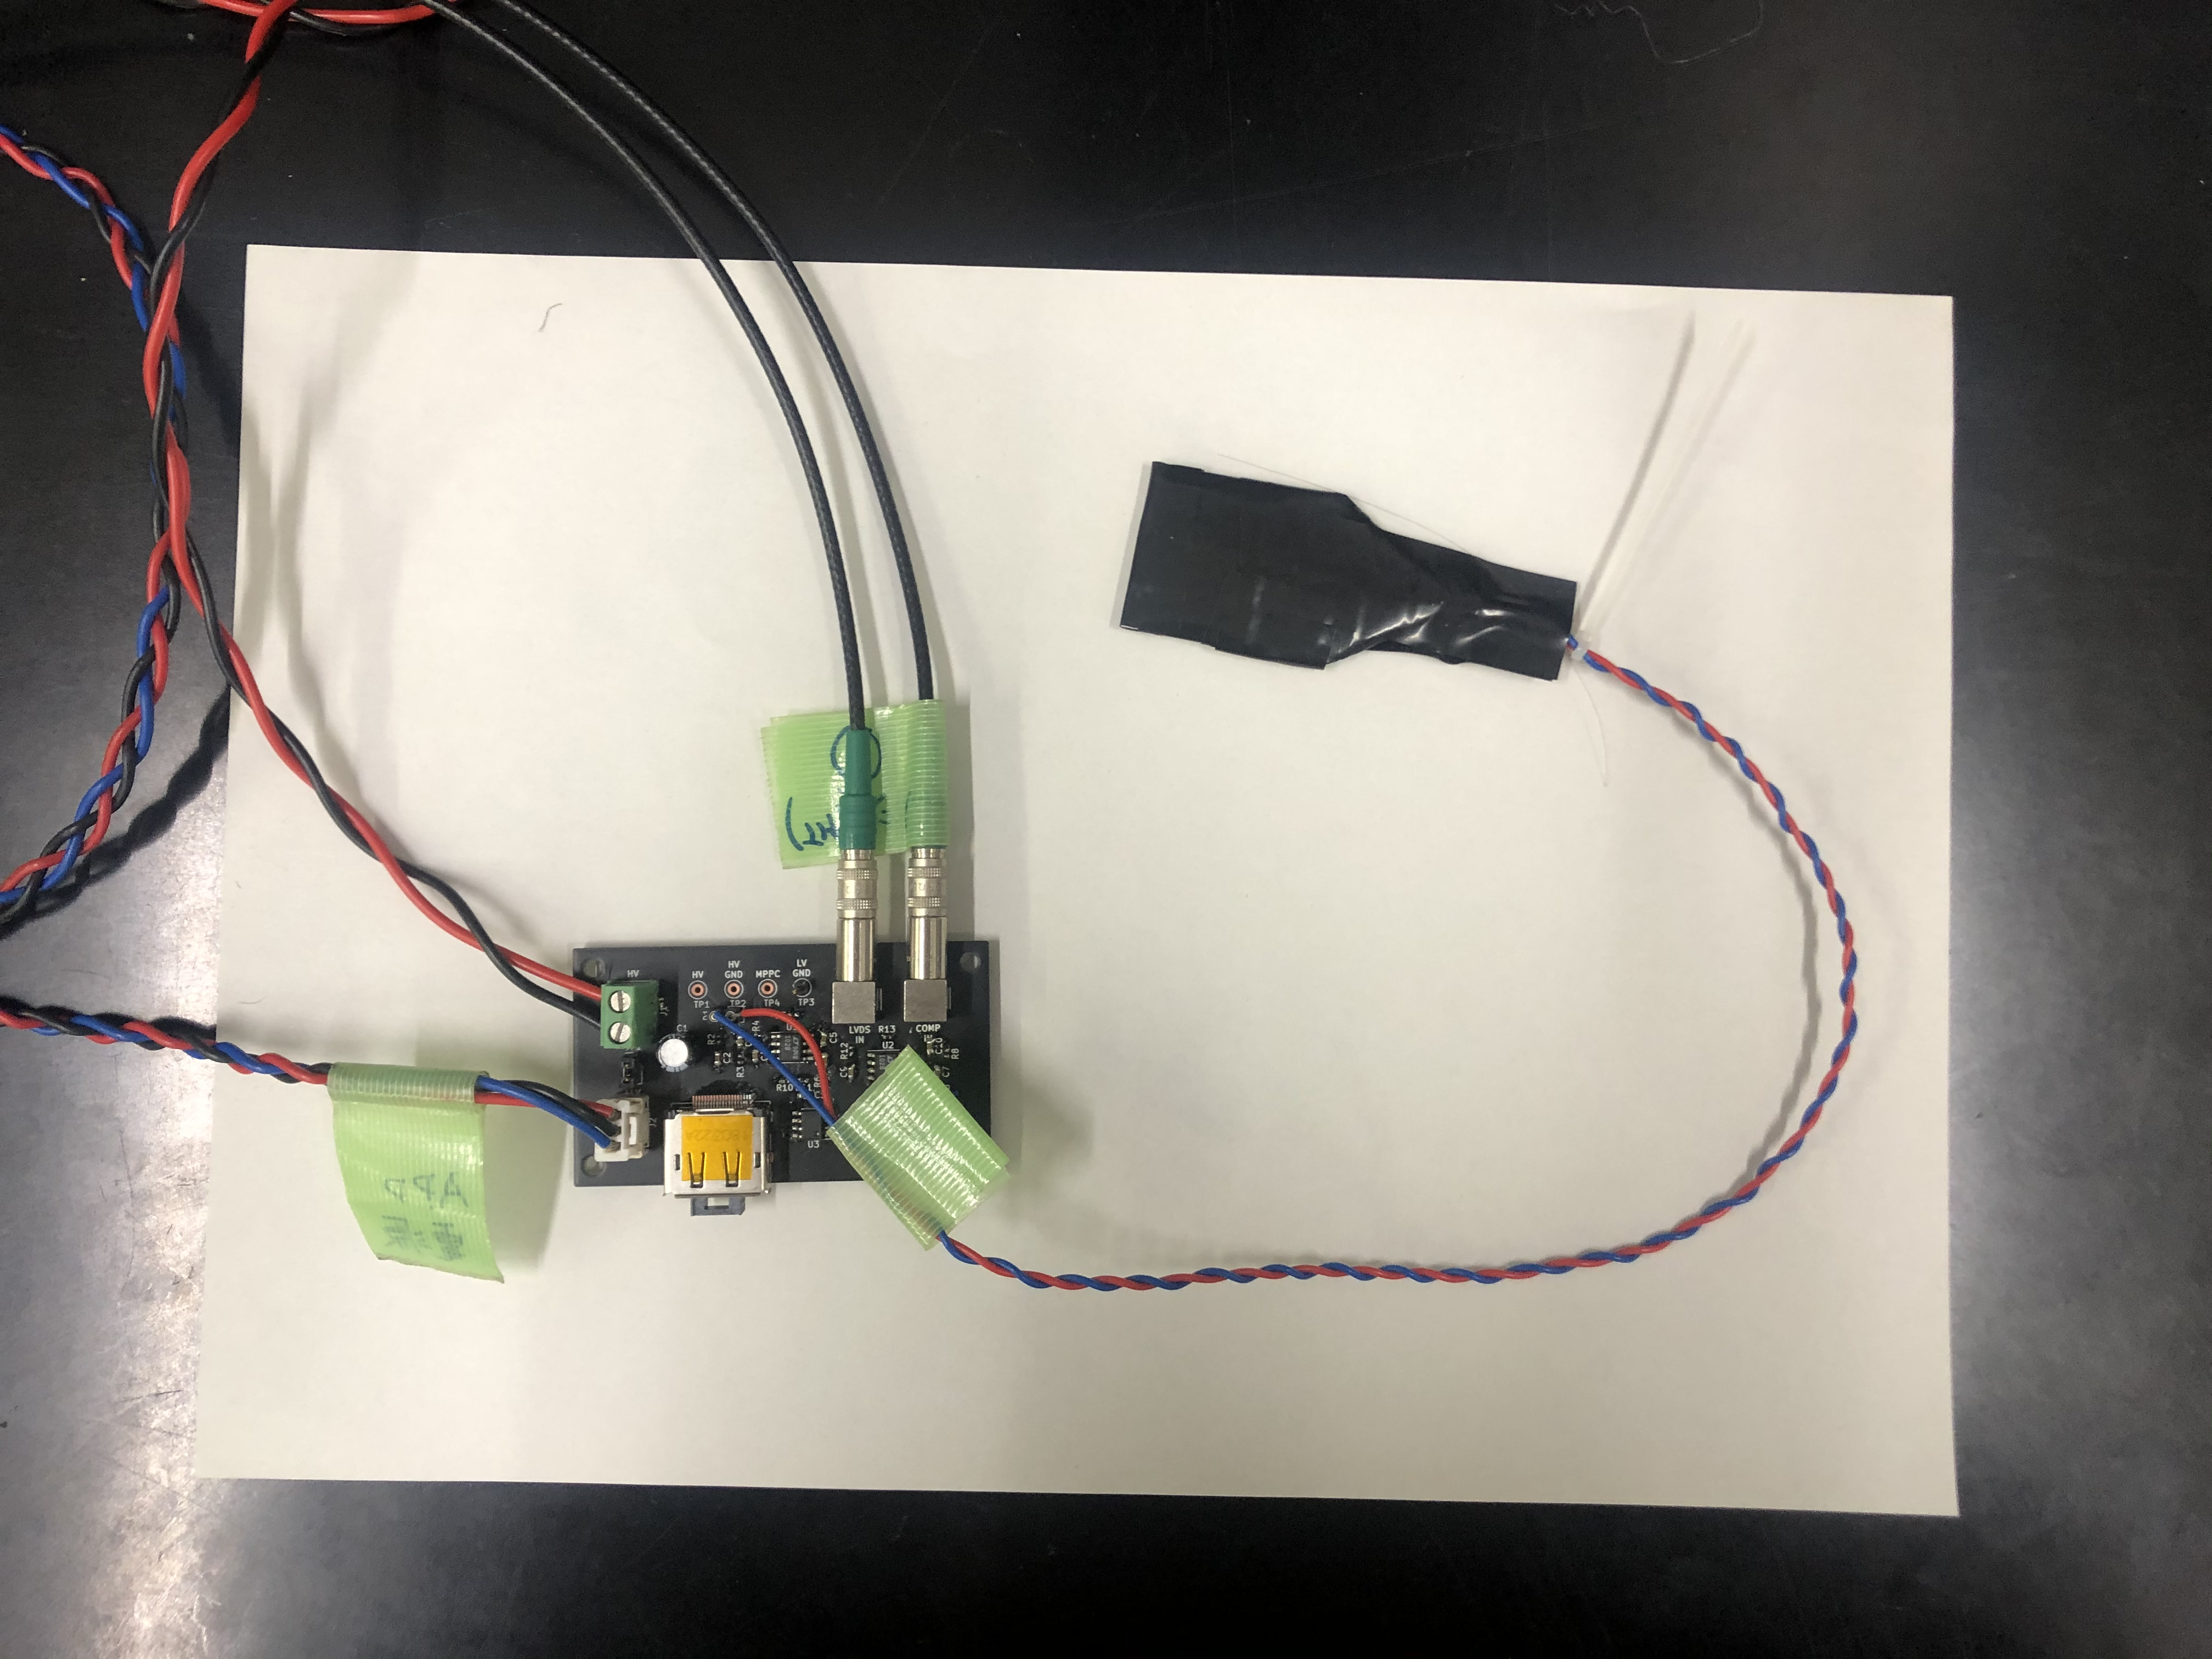
\includegraphics[width=15cm]{./figure/trigsetup.png}
%  \caption{トリガシンチの基礎測定セットアップ}
%  \label{fig:trigsetup}
%\end{figure}
%
%\subsubsection*{トリガシンチの信号を波形整形する基板}
%本研究を行うにあたって,MPPCからの信号を波形整形する基板を作成した.基板を図\ref{fig:extcircle}に示す.主に,電圧供給回路,反転増幅回路,コンパレータ回路,LVDS変換回路から構成されている.基板はKiCADというCERN開発のオープンソースプリント基板CADを用いて設計・作成した.LEMO1からは増幅されたMPPCのアナログ信号を,LEMO2からはコンパレータによって閾値電圧と比較することで変換されたデジタル信号を,DPからはTTLだったデジタル信号が変換されてLVDS出力のデジタル信号を読み出すことができる.その3点についてオシロスコープで観測した波形を図\ref{fig:extosiro}に示す.基礎測定では,LEMO2の出力からGATE信号を生成し,LEMO1の出力のデータを測定した.
%
%\begin{figure}[h]
%  \centering
%  \begin{minipage}[b]{0.45\linewidth}
%    \centering
%    \includegraphics[width=6cm]{./figure/trigscin.png}
%    \subcaption{基板の様子}
%    \label{fig:pcb}
%  \end{minipage}
%  \begin{minipage}[b]{0.45\linewidth}
%    \centering
%    \includegraphics[width=8cm]{./figure/pcbosiro.png}
%    \subcaption{動作確認したオシロスコープの様子}
%    \label{fig:extosiro}
%  \end{minipage}
%  \caption{トリガシンチの信号を波形整形する基板}
%\end{figure}
%
%\subsection{光量と粒子の入射位置の依存性測定}
%粒子の入射位置がMPPCから最も離れている時と,最も近い時で,トリガシンチの読み出す光量にどれくらいの差が出るのかをライトガイドがある場合とない場合で測定した.ライトガイドの必要性を評価するためにこの測定を行なった.
%
%\subsubsection*{手順}
%測定を行なった時のトリガシンチと粒子の入射位置を図\ref{fig:trigscinlg}に示す.粒子の入射位置は,トリガシンチと線源の間に小さな穴の空いた鉄板を設置することで調節した.鉄板の穴の位置がMPPCから最も離れている時(図中A)と,最も近い時(図中B)で,トリガシンチから読み出された光量を測定した.ライトガイドありの場合となしの場合で,位置による光量の差に変化があるかを測定した.コンパレータの比較電圧$V_{ref}$を150 $\mathrm{mV}$に設定した.
%
%\begin{figure}[h]
%  \centering
%  \begin{minipage}[b]{0.45\linewidth}
%    \centering
%    \includegraphics[height=2cm]{./figure/trigscinwlg.png}
%    \subcaption{ライトガイドがある場合}
%    \label{fig:trigscinwlg}
%  \end{minipage}
%  \begin{minipage}[b]{0.45\linewidth}
%    \centering
%    \includegraphics[height=2cm]{./figure/trigscinwolg.png}
%    \subcaption{ライトガイドがない場合}
%    \label{fig:trigscinwolg}
%  \end{minipage}
%  \caption{トリガシンチと粒子の入射位置の関係}
%  \label{fig:trigscinlg}
%\end{figure}
%
%\subsubsection*{結果}
%測定結果は図\ref{fig:trigscincon}のようになっている.
%
%\begin{figure}[h]
%  \centering
%  \begin{minipage}[b]{0.45\linewidth}
%    \centering
%    \includegraphics[width=7.5cm]{./figure/trigscinwlgcon.png}
%    \subcaption{ライトガイドがある場合}
%    \label{fig:trigscinwlg}
%  \end{minipage}
%  \begin{minipage}[b]{0.45\linewidth}
%    \centering
%    \includegraphics[width=7.5cm]{./figure/trigscinwolgcon.png}
%    \subcaption{ライトガイドがない場合}
%    \label{fig:trigscinwolg}
%  \end{minipage}
%  \caption{トリガシンチと粒子の入射位置の関係}
%  \label{fig:trigscinlgcon}
%\end{figure}
%
%
%
%\subsection{トリガレートの測定}
%トリガシンチの上に線源を配置した時としない時で,どれくらい
%\subsubsection*{手順}
%トリガシンチの上に線源を配置した時としない時で,100000イベントのデータを取得するのにかかる時間を測定した.
%
%\subsubsection*{結果}
%トリガシンチの上に線源を配置した時としない時のトリガレートの比較結果は表\ref{tab:trigscinrate}のようになっている.
%
%\
%
%
%
%\section{外部トリガを用いた応答評価試験セットアップ}
%\label{sec:extsetup}
%RD53Aの量産にあたって,行われる品質試験では,外部トリガを用いた応答評価試験が行われる.そのため,実際に行われる試験環境に近いセットアップで試験を行なった.セットアップの写真を以下に示す.MPPCには58$\mathrm{V}$印加した.SCCとFPGAボード,PCを用いてシステムを組む大枠は変わらずに,線源の配置とトリガに使用するものが異なっている.\par
%実際に行われる試験は,クーリングボックスと呼ばれる,温度が低温に維持された小さな箱の中で行い,トリガには前章で述べたHitOR信号ではなく,シンチレータからの光信号を用いる.シンチレータは線源とモジュールの間に設置するため,なるべく$\beta$線を遮らないように,厚みは0.5$\mathrm{mm}$と非常に薄いものを使用した.
%実際に行われる試験環境はクーリングボックスと呼ばれる,温度が低温に維持された小さな箱の中で行う.それに合う応答評価試験セットアップを考えるにあたって,線源とシンチレータ,シンチレータの光信号を電気信号に変換するMPPCが乗ったソースホルダと,MPPCからのアナログ信号を波形整形し,LVDSのデジタル信号に変換するような基板の設計を行なった.
%
%\subsection{ソースホルダの設計}
%ソースホルダの外観を以下に示す.クーリングボックス内で使用することを想定し,コンパクトな作りになっている.これは,FreeCADというオープンソース汎用3D CADモデラで設計し,3Dプリンタを用いて作成した.
%
%\subsection{MPPCからの信号を波形整形する回路}
%
%\subsubsection*{回路の動作確認}
%MPPCからの信号を正しく波形整形できているかをオシロスコープを用いて確認した.増幅されたMPPCからの信号がコンパレータによって,デジタル信号に変換され,TTL to LVDS変換のチップによって,差動信号に変換されている様子がわかる.
%
%\section{トリガシンチの基礎測定}
%この回路では,信号を出力をコンパレータの閾値によって設定している.この閾値によって,MPPCからの信号が削られることなく伝達されているかを確認した.
%
%\section{応答評価試験手順}
%\label{sec:exthow}
%\section{応答評価試験結果}
%\label{sec:extconc}
%\section{考察}
%\label{sec:extsum}

\chapter{2つの手法で行なった応答評価試験の比較}
この章では,第4章,第5章で述べた,セルフトリガと外部トリガ,それぞれを用いた応答評価試験の結果から,それぞれの手法の比較を行う.

\section{全トリガ数に対するヒットが存在したイベント数}
セルフトリガと外部トリガ,それぞれを用いた応答評価試験で得られた全トリガ数のうちのヒット数が存在したイベント数の分布を表\ref{tab:selfrcomp},表\ref{tab:extrcomp}に示す.

\begin{table}[h]
  \centering
  \caption{セルフトリガの場合の全トリガ数と対するヒットが存在したイベント数の割合}
  \begin{tabular} {l|ccc} \hline
    time:1800[sec] & $M^{\mathrm{self}}$ & $M_{\mathrm{data}}^{\mathrm{self}}$ & $M_{\mathrm{emp}}^{\mathrm{self}}$ \\ \hline \hline
    トリガ数 & 4056311 & 3528141 & 528170 \\
     & (100 \%) & (87.0 \%) & (13.0 \%) \\ \hline
    トリガ数/time & 2254 $\mathrm{Hz}$ & 1960 $\mathrm{Hz}$ & 293.4 $\mathrm{Hz}$ \\ \hline
  \end{tabular}
  \label{tab:selfrcomp}
\end{table}

\begin{table}[h]
  \centering
  \caption{外部トリガの場合の全トリガ数と対するヒットが存在したイベント数の割合}
  \begin{tabular} {l|ccc} \hline
    time:1800[sec] & $M^{\mathrm{ext}}$ & $M_{\mathrm{data}}^{\mathrm{ext}}$ & $M_{\mathrm{emp}}^{\mathrm{ext}}$ \\ \hline \hline
    トリガ数 & 918246 & 278687 & 639559 \\
     & (100 \%) & (30.3 \%) & (69.7 \%) \\ \hline
    トリガ数/time & 85.0 $\mathrm{Hz}$ & 25.8 $\mathrm{Hz}$ & 59.2 $\mathrm{Hz}$ \\ \hline
  \end{tabular}
  \label{tab:extrcomp}
\end{table}

セルフトリガで取得したデータは,83 \%のイベントにヒットが存在する一方で,外部トリガで取得したデータは,23 \%のイベントにしかヒットが存在しない.原理として,セルフトリガは荷電粒子がセンサを通過した信号由来でトリガを生成しているのに対し,外部トリガは,トリガシンチレータを荷電粒子が通過した信号由来でトリガを生成しているため,このようなヒットの存在率に差ができると考えられる.

\section{平均の1ピクセルあたりのヒット数}
セルフトリガと外部トリガ,それぞれを用いた応答評価試験で得られた結果から求めた,平均の1ピクセルあたりのヒット数は以下のようになる.

\begin{itemize}
\item セルフトリガ:15.1 $\mathrm{Hits/pixel/30min}$\\
\item 外部トリガ:1.10 $\mathrm{Hits/pixel/3h}$
\end{itemize}

これより求められる,各ピクセル50 $\mathrm{Hits/pixe}$を得て,品質評価を行うために必要な時間は以下のようになる.
\begin{itemize}
\item セルフトリガ:100 $\mathrm{min}$\\
\item 外部トリガ:6.25 $\mathrm{day}$
\end{itemize}

どちらも,実際2000個のモジュールに対して応答評価試験を行うことを考えると,大変長く,現実味のない値である.実際の試験では,外部トリガを用いた応答評価試験を行う予定であるが,時間を短縮するために,本論文で用いた4.8 $\mathrm{kBq}$の線源よりも1000倍強い放射能を持った線源を使用する必要があると考える.1000倍強い線源を使用することで,1モジュールあたり9分で応答評価試験が終えられると予測される.

\section{全ヒット数に対する荷電粒子のヒット数}
セルフトリガと外部トリガ,それぞれを用いた応答評価試験で得られた結果から求めた荷電粒子のヒット数の分布を表\ref{tab:selfpcomp},表\ref{tab:extpcomp}に示す

\begin{table}[h]
  \centering
  \caption{セルフトリガで得られた荷電粒子のヒット数}
  \begin{tabular} {l|ccc} \hline
    time:1800[sec]& $N^{\mathrm{self}}$ & $N_{\mathrm{bg}}^{\mathrm{self}}$ & $N_{\mathrm{sig}}^{\mathrm{self}}$ \\ \hline \hline
    ヒット数 & 3599457 & 2954185 & 645272 \\
    & (100 \%) & (82.1 \%) & (17.9 \%) \\ \hline
    ヒット数/time & 1999.7 $\mathrm{Hz}$ & 1641.2 $\mathrm{Hz}$ & 358.5 $\mathrm{Hz}$ \\ \hline
  \end{tabular}
  \label{tab:selfpcomp}
\end{table}

\begin{table}[h]
  \centering
  \caption{外部トリガで得られた荷電粒子のヒット数}
  \begin{tabular} {l|ccc} \hline
    time:10800[sec]& $N^{\mathrm{ext}}$ & $N_{\mathrm{bg}}^{\mathrm{ext}}$ & $N_{\mathrm{sig}}^{\mathrm{ext}}$ \\ \hline \hline
    ヒット数 & 591115 & 4620 & 586495 \\
    & (100 \%) & (0.8 \%) & (99.2 \%) \\ \hline
    ヒット数/time & 54.7 $\mathrm{Hz}$ & 0.9 $\mathrm{Hz}$ & 54.3 $\mathrm{Hz}$ \\ \hline
  \end{tabular}
  \label{tab:extpcomp}
\end{table}

 
全ヒット数に含まれる荷電粒子のヒット数は外部トリガの方が良いが,ヒットレートについては,セルフトリガの方が良い結果となっている.これより,取得されるデータの容量を考慮しないのであれば,セルフトリガの手法がよく,少ないデータ容量で荷電粒子のヒットを得たい場合は外部トリガを使用する方が良いと考えられる.


%\section{ヒットが得られたピクセルに対する荷電粒子の信号検出効率}
%この節では,ヒットが得られたピクセルに対する荷電粒子の信号検出効率を述べる.荷電粒子からの信号の検出効率を比較するために,ヒットが存在したピクセルに対する荷電粒子によるヒットが得られたピクセルの割合を,セルフトリガと外部トリガ,それぞれの場合で比較する.ここでは,表\ref{tab:patern}のようにa,bの場合を定める.
%\begin{table}[h]
%  \centering
%  \begin{tabular}{c|cc} \hline
%    & 線源なしの時 & 線源ありの時 \\ \hline
%    a & ヒットなし & ヒットあり\\
%    b & ヒットあり & ヒットあり \\ \hline
%  \end{tabular}
%\end{table}
%
%表\ref{tab:conc4}は,第4章と第5章の結果をまとめたものである.
%\begin{table}[h]
%  \centering
%  \begin{tabular}{cc|c|c}\hline
%    & & セルフトリガ & 外部トリガ \\ \hline
%    $a_{\mathrm{ALL}}$ & aのピクセル数 & 22910 & 9369 \\
%    $b_{\mathrm{ALL}}$ & bのピクセル数 & 957 & 24 \\
%    $a_{\mathrm{sig}}$ & aの中で荷電粒子からの信号を検出できたピクセル & 22854 & 9369 \\
%    $b_{\mathrm{sig}}$ & bの中で荷電粒子からの信号を検出できたピクセル & 880 & 8 \\ \hline
%  \end{tabular}
%\end{table}
%
%この時,ヒットが存在したピクセルに含まれる荷電粒子からのヒットが存在したピクセルの割合は以下のように求められる.
%
%\begin{eqnarray}
%  \label{eq:sigma}
%  \frac{a_{\mathrm{sig}} + b_{\mathrm{sig}}}{a_{\mathrm{ALL}} + b_{\mathrm{ALL}}} &\pm& \sigma\\
%  \sigma &=& \sqrt{\sigma_{a}^2 + \sigma_{b}^2 + \sigma_{c}^2 + \sigma_{d}^2} \\ \nonumber
%  \sigma_a &=& \frac{1}{a_{\mathrm{ALL}} + b_{\mathrm{ALL}}} \sqrt{a_{\mathrm{sig}}}\\ \nonumber
%  \sigma_b &=& \frac{1}{a_{\mathrm{ALL}} + b_{\mathrm{ALL}}} \sqrt{b_{\mathrm{sig}}}\\ \nonumber
%  \sigma_c &=& \frac{a_{\mathrm{sig}} + b_{\mathrm{sig}}}{\left(a_{\mathrm{ALL}} + b_{\mathrm{ALL}}\right)^2}\sqrt{a_{\mathrm{ALL}}}\\ \nonumber
%  \sigma_d &=& \frac{a_{\mathrm{sig}} + b_{\mathrm{sig}}}{\left(a_{\mathrm{ALL}} + b_{\mathrm{ALL}}\right)^2}\sqrt{b_{\mathrm{ALL}}}\\ \nonumber
%\end{eqnarray}
%
%式\ref{eq:sigma}より,セルフトリガと外部トリガの場合のヒットが存在したピクセルに含まれる荷電粒子からのヒットが存在したピクセルの割合は
%\begin{itemize}
%\item セルフトリガ:0.994 $\pm$ 0.00912 
%\item 外部トリガ:0.998 $\pm$ 0.0145
%\end{itemize}
%
%となり,セルフトリガと外部トリガで割合は一致した.すなわち,線源を置いた時にヒットがあったピクセルについては,どちらの手法でも,約99\%のピクセルが荷電粒子による信号を検出できているということがわかった.\par
%しかし,セルフトリガでは,センサからのノイズでトリガをかけて取得されたデータも多い.そのため,線源なしの時にも線源ありの時にもヒットが存在するピクセルが,外部トリガの時よりも多く存在する.
%
%
%\section{データの取得効率}
%この節では,2つの手法のデータ取得効率について述べる.データの取得効率を比較するために,トリガ数に対するヒットの存在したイベント数の割合を表\ref{tab:conc1}に示す.セルフトリガで取得したデータはトリガ数に対して約85 \%,外部トリガで取得したデータはトリガ数に対して約29 \%のデータ取得効率であった.これより,セルフトリガで取得されたデータの方が外部トリガでデータを取得するよりも,データ取得効率が良いことがわかる.
%
%\begin{table}[h]
%  \centering
%  \caption{ヒット数0のイベント数/トリガ数}
%  \label{tab:conc1}
%  \begin{tabular}{c|cc|cc} \hline
%    & \multicolumn{2}{c|}{セルフトリガ} & \multicolumn{2}{c}{外部トリガ} \\
%    & 線源なし & 線源あり & 線源なし & 線源あり \\ \hline
%    トリガ数 & 4193686 & 4056311 & 29353 & 918246 \\
%    ヒットの存在したイベント数 & 3528141 & 3481776 & 8446 & 278687 \\
%    割合[\%] & 84.1 & 85.8 & 28.8 & 30.3 \\ \hline
%  \end{tabular}
%\end{table}
%
%また,線源を置いた時にヒットが得られなかったピクセルの数の比較を表\ref{fig:conc2}に示す.外部トリガの時よりもセルフトリガの時の方が,荷電粒子によるヒットが得られなかったピクセルの数が少なく.ほとんどのピクセルにヒットがあることがわかる.図\ref{fig:selfo},図\ref{fig:extw}のヒットの分布を見ても,セルフトリガの場合は全面いヒットが見られ,外部トリガの場合は0ヒットのピクセルが多く分布しているのが確認できる.
%
%\begin{table}[h]
%  \centering
%  \caption{ヒットが得られなかったピクセルの数}
%  \begin{tabular}{c|c|c} \hline
%    & セルフトリガ & 外部トリガ \\ \hline
%    ヒットが得られなかったピクセル数 & 15 & 14489 \\ \hline
%  \end{tabular}
%\end{table}
%
%以上より,セルフトリガでデータ取得をした方が,外部トリガでデータ取得を行なった時よりも,データ取得効率はいいと考えられる.外部トリガでデータ取得を行って,今回使用した23882ピクセル全部に荷電粒子を当てることを考える.今回ヒットが存在したピクセル数9393より,$23882/9393 = 2.54$となるので,今回使用した$4.8 \mathrm{kBq}$の線源の10倍ほど強い線源を用いれば,今回よりも短時間で効率の良い応答評価試験が行えると考える.
%
%
%


\chapter*{謝辞}

本研究を進める上でお世話になった方々にお礼申し上げます.指導教員である河野能知准教授には,研究の機会と環境を与えていただきました.また,素粒子実験に関わる知識だけでなくファームウェア,ソフトウェア,回路設計などのノウハウや,研究発表にあたって見やすく伝わりやすい資料作りについてご指導いただきました.毎週の研究室のミーティングでは,研究方針および手法について的確な指摘をいただき,研究をすすめることができました.心から感謝申し上げます.また,副指導教員で本論文の副査を務めていただきました高橋遼助教授にも感謝申し上げます.\par
ATLAS日本QA/QCグループの皆様に感謝いたします.大阪大学の廣瀬穣さんには,ミーティングの場だけでなく,ミーティング外でも時間をとって,ファームウェアの知識のない私に丁寧にご指導いただきましたことに感謝申し上げます.また,東京工業大学の生出秀行さんにも,ソフトウェアの開発やソースホルダの作成の際にたくさんのアドバイスをいただきました.感謝いたします.また,東工大の窪田ありささん,阪大の山家谷昌平さんには,同期として研究姿勢について多くを学ばせていただきました.東工大の松崎貴由さん.池亀遥南さんには,クーリングボックスにソースホルダを組み込むにあたって設計についての相談にのっていただきました.東工大の奥山広貴さんにはデータベースの使い方を丁寧に教えていただき,また阪大のLakmin Wickremasingheさんには回路設計についてアドバイスをいただきました.\par
お茶の水女子大学河野研究室の皆様に感謝申し上げます.藤本みのりさんには,データ取得を手伝っていただいたこと,ファームウェアとソフトウェアについての多くの知識を教えていただきました.浅井香奈江さんには,コーディング技術や,プロットの見せ方について多くの助言をいただきました.河野研究室卒業生の里吉陽奈子さんには,見やすい発表資料の作り方について大変参考にさせていただきました.また修士1年で同じATLAS日本QA/QCグループだった,釣希夢さん,前田実津季さんには発表資料や実験方針,ソフトウェアの設計など,多くの相談にのっていただき,大変感謝しています.\par
ATLASグループでは,KEKの中村浩二さん,筑波大学の原田大豪さんには,センサについての知識を教えていただいた上に,データ取得するにあたって多くの時間をとって協力してくださり大変感謝しています.また,東工大の金恩寵さん,潮田理沙さん,卒業生の中村優斗さんには学会などで会うたびによくしてくだいました.ありがとうございました.\par
最後に,何不自由ない学生生活,研究生活を実現してくたださった両親に深く感謝いたします.




\bibliography{./bib/IOPEXPORT_BIB}
\bibliographystyle{junsrt}
%\bibliography{./bib/HLLHC_BIB}
%\bibliography{./bib/ITK_BIB}

\appendix

\listoffigures
\listoftables

\end{document}

